\section{The Plutus Platform}

The \gls{plutus-platform} is a platform for writing \emph{applications} that interact with a \emph{distributed ledger} featuring \emph{scripting capabilities}, in particular the \gls{cardano} blockchain.
A high-level architecture of the \gls{plutus-platform} on \gls{cardano} is shown in \cref{fig:platform-architecture}, with an emphasis on applications.

\paragraph{Ledgers.}
The \gls{plutus-platform} is designed to work with distributed ledgers (henceforth simply ``ledgers'').\footnote{
More specifically, it is designed to work with the \gls{cardano} blockchain, although it could function on other systems that implement the requisite ledger functionality.
}
While the design of the Platform supports writing very simple applications that do nothing but occasionally submit money-transfer transactions to the ledger,
 the main focus is on the applications which are enabled by a ledger with scripting functionality.
Specifically, we look at \gls{utxo} ledgers which implement what we call the \gls{eutxo-model}.

The ledger model is described in \cref{sec:ledger}.

\paragraph{Scripting.}
Ledgers without scripting functionality can only support very simple applications.
Much of the interest in applications that interact with blockchains has come from the ability to put some part of the application code \emph{on} the chain itself (such code is generally referred to as a ``\gls{script}''), such that it is guaranteed to be executed correctly as part of the consensus protocol of the blockchain.
This enables applications to have small kernels of ``trusted'' code which ensures that critical safety conditions are met.

The \gls{plutus-platform} requires a particular scripting model from the ledger, which is described with the general ledger model in \cref{sec:ledger}.
This scripting model is agnostic about the scripting \emph{language} which is used for \glspl{script}, but the \gls{plutus-sdk} is designed to work with a particular scripting language, namely \gls{plutus-core}. \Gls{plutus-core} is described in \cref{sec:plutus-core}.

\paragraph{Applications.}
What is a ``\gls{app}''?
In the \gls{plutus-platform} a \gls{app} is simply a program that interacts with a distributed ledger.
We use the rather generic word ``application'' over the more usual ``smart contract'' or ``distributed application'' to emphasize the generic nature of the programs we are considering --- indeed, they may not use the scripting functionality of the ledger at all!

The point of the Platform is to enable such applications by providing support in the ledger, as well as support for authoring, distributing, and running them.
While the modifications to the ledger may seem like the most technically substantive part of the work, most of the application behaviour is in the part that runs off the chain, and this requires a commensurate amount of support.

The \gls{app} model is described in \cref{sec:paf}, and our support for authoring \glspl{app} in \cref{sec:sdk}.

\begin{figure}[t]
  \centering
  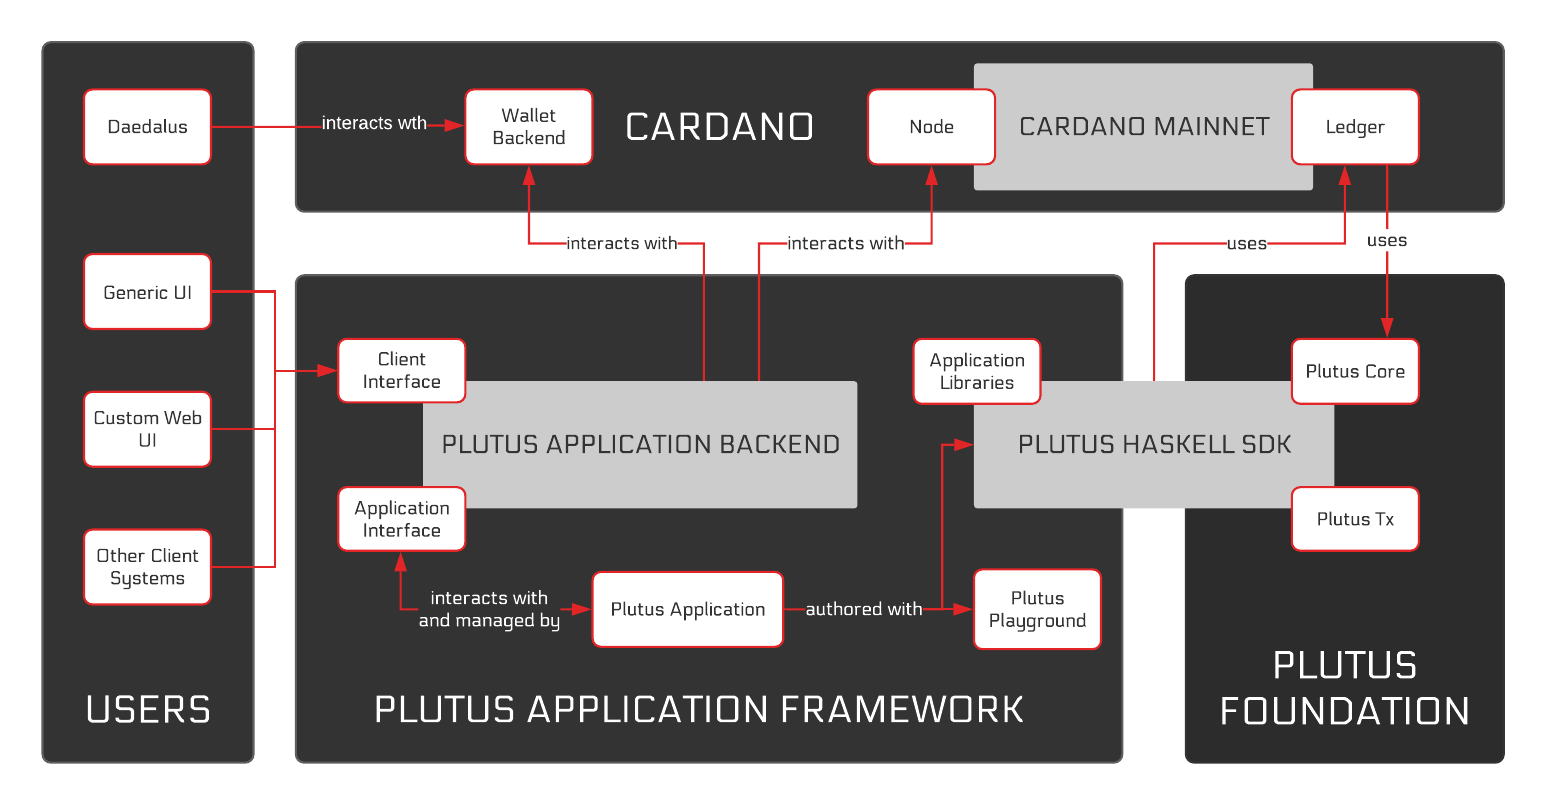
\includegraphics[width=\textwidth]{platform-architecture.png}
  \caption{Architecture of the \gls{plutus-platform}}
  \label{fig:platform-architecture}
\end{figure}
